\documentclass[14pt, a4paper]{report}
\usepackage{mathtext}
\usepackage[T2A]{fontenc}
\usepackage[utf8]{inputenc}
\usepackage[russian]{babel}
\usepackage{multirow}
\usepackage{slashbox}
\usepackage{makecell}
\usepackage{graphicx}
\usepackage{physics}
\usepackage{amstext}
\usepackage{caption}
\usepackage{subcaption}
\usepackage{cmap}
\usepackage{float}
\usepackage{indentfirst}
\usepackage{romannum}

\usepackage[a4paper,
            		left=1in,
            		right=1in,
           		 top=1in,
            		bottom=1in,
            		footskip=.25in]{geometry}

\renewcommand{\thesection}{\arabic{section}.}
\renewcommand{\thesubsection}{\arabic{section}.\arabic{subsection}.}

\title{\textbf{Отчет о выполнении лабораторной работы 5.8.1 "Определение постоянных Стефана-Больцмана и Планка из анализа теплового излучения нагретых тел"}}
\author{Калашников Михаил, Б03-202}
\date{}

\begin{document}
\maketitle

\pagenumbering{arabic}

\section{Теоретические сведения}

Для измерения температуры разогретых тел, удаленных от наблюдателя, применяют методы оптической пирометрии, основанные на использовании зависимости испускательной способности исследуемого тела от температуры. Различают три температуры, функционально связанные с истинной термодинамической температурой и излучательной способностью тела: радиационную, цветовую и яркостную.

Под радиационной (энергетической) температурой понимают температуру абсолютно черного тела, при которой его интегральная испускательная способность одинакова с интегральной испускательной способностью исследуемого тела.

Под цветовой температурой исследуемого тела понимают температуру абсолютно черного тела, при которой отношение их спектральных испускательных способностей для двух заданных длин волн одинаково.

Под яркостной температурой понимают температуру абсолютно черного тела, при которой его спектральная испускательная способность равна спектральной испускательной способности исследуемого тела при той же длине волны. Именно эту температуру мы будем измерять в данной работе.

\section{Экспериментальная установка}

\begin{figure}[H]
\centering
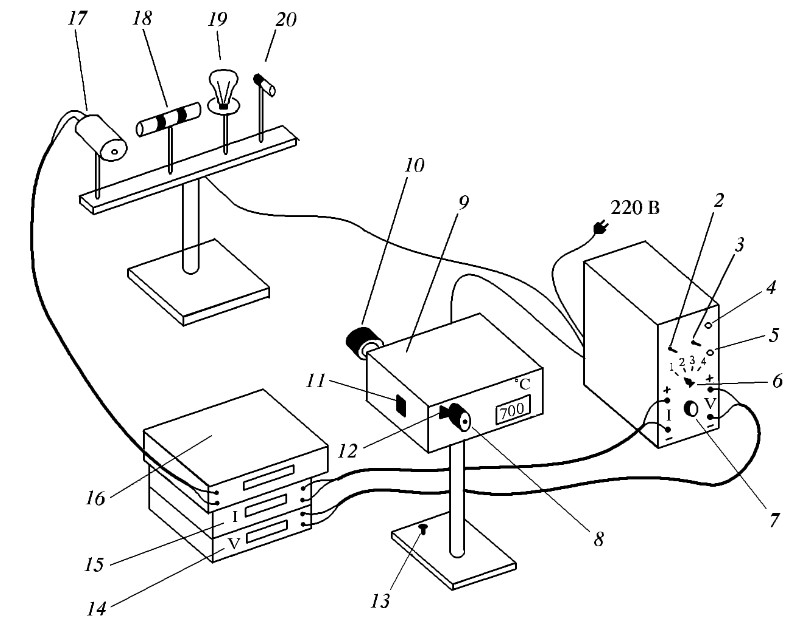
\includegraphics[width=.8\linewidth]{../images/581-5}
\caption{Схема экспериментальной установки: 1 -- блок питания; 2 -- тумблер включения питания пирометра и образцов; 3 -- тумблер нагрева нити пирометра:  «Быстро» -- вверх,  «Медленно» -- вниз; 4 -- кнопка  «Нагрев нити»; 5 -- кнопка  «Охлаждение нити»; 6 -- тумблер переключения образцов; 7 -- регулятор мощности нагрева образцов; 8 -- окуляр пирометра; 9 -- корпус пирометра; 10 -- объектив пирометра; 11 -- переключение диапазонов: 700-1200 -- вниз, 1200-2000 -- вверх; 12 -- ручка перемещения красного светофильтра; 13 -- регулировочный винт; 14 -- вольтметр (напряжение на лампе накаливания); 15 -- амперметр (ток через образ-
цы); 16 -- вольтметр в цепи термопары; 17 -- модель АЧТ; 18 -- трубка с кольцами из материалов с разной излучательной способностью; 19 -- лампа накаливания; 20 -- неоновая лампочка}
\end{figure}

\begin{figure}[H]
\centering
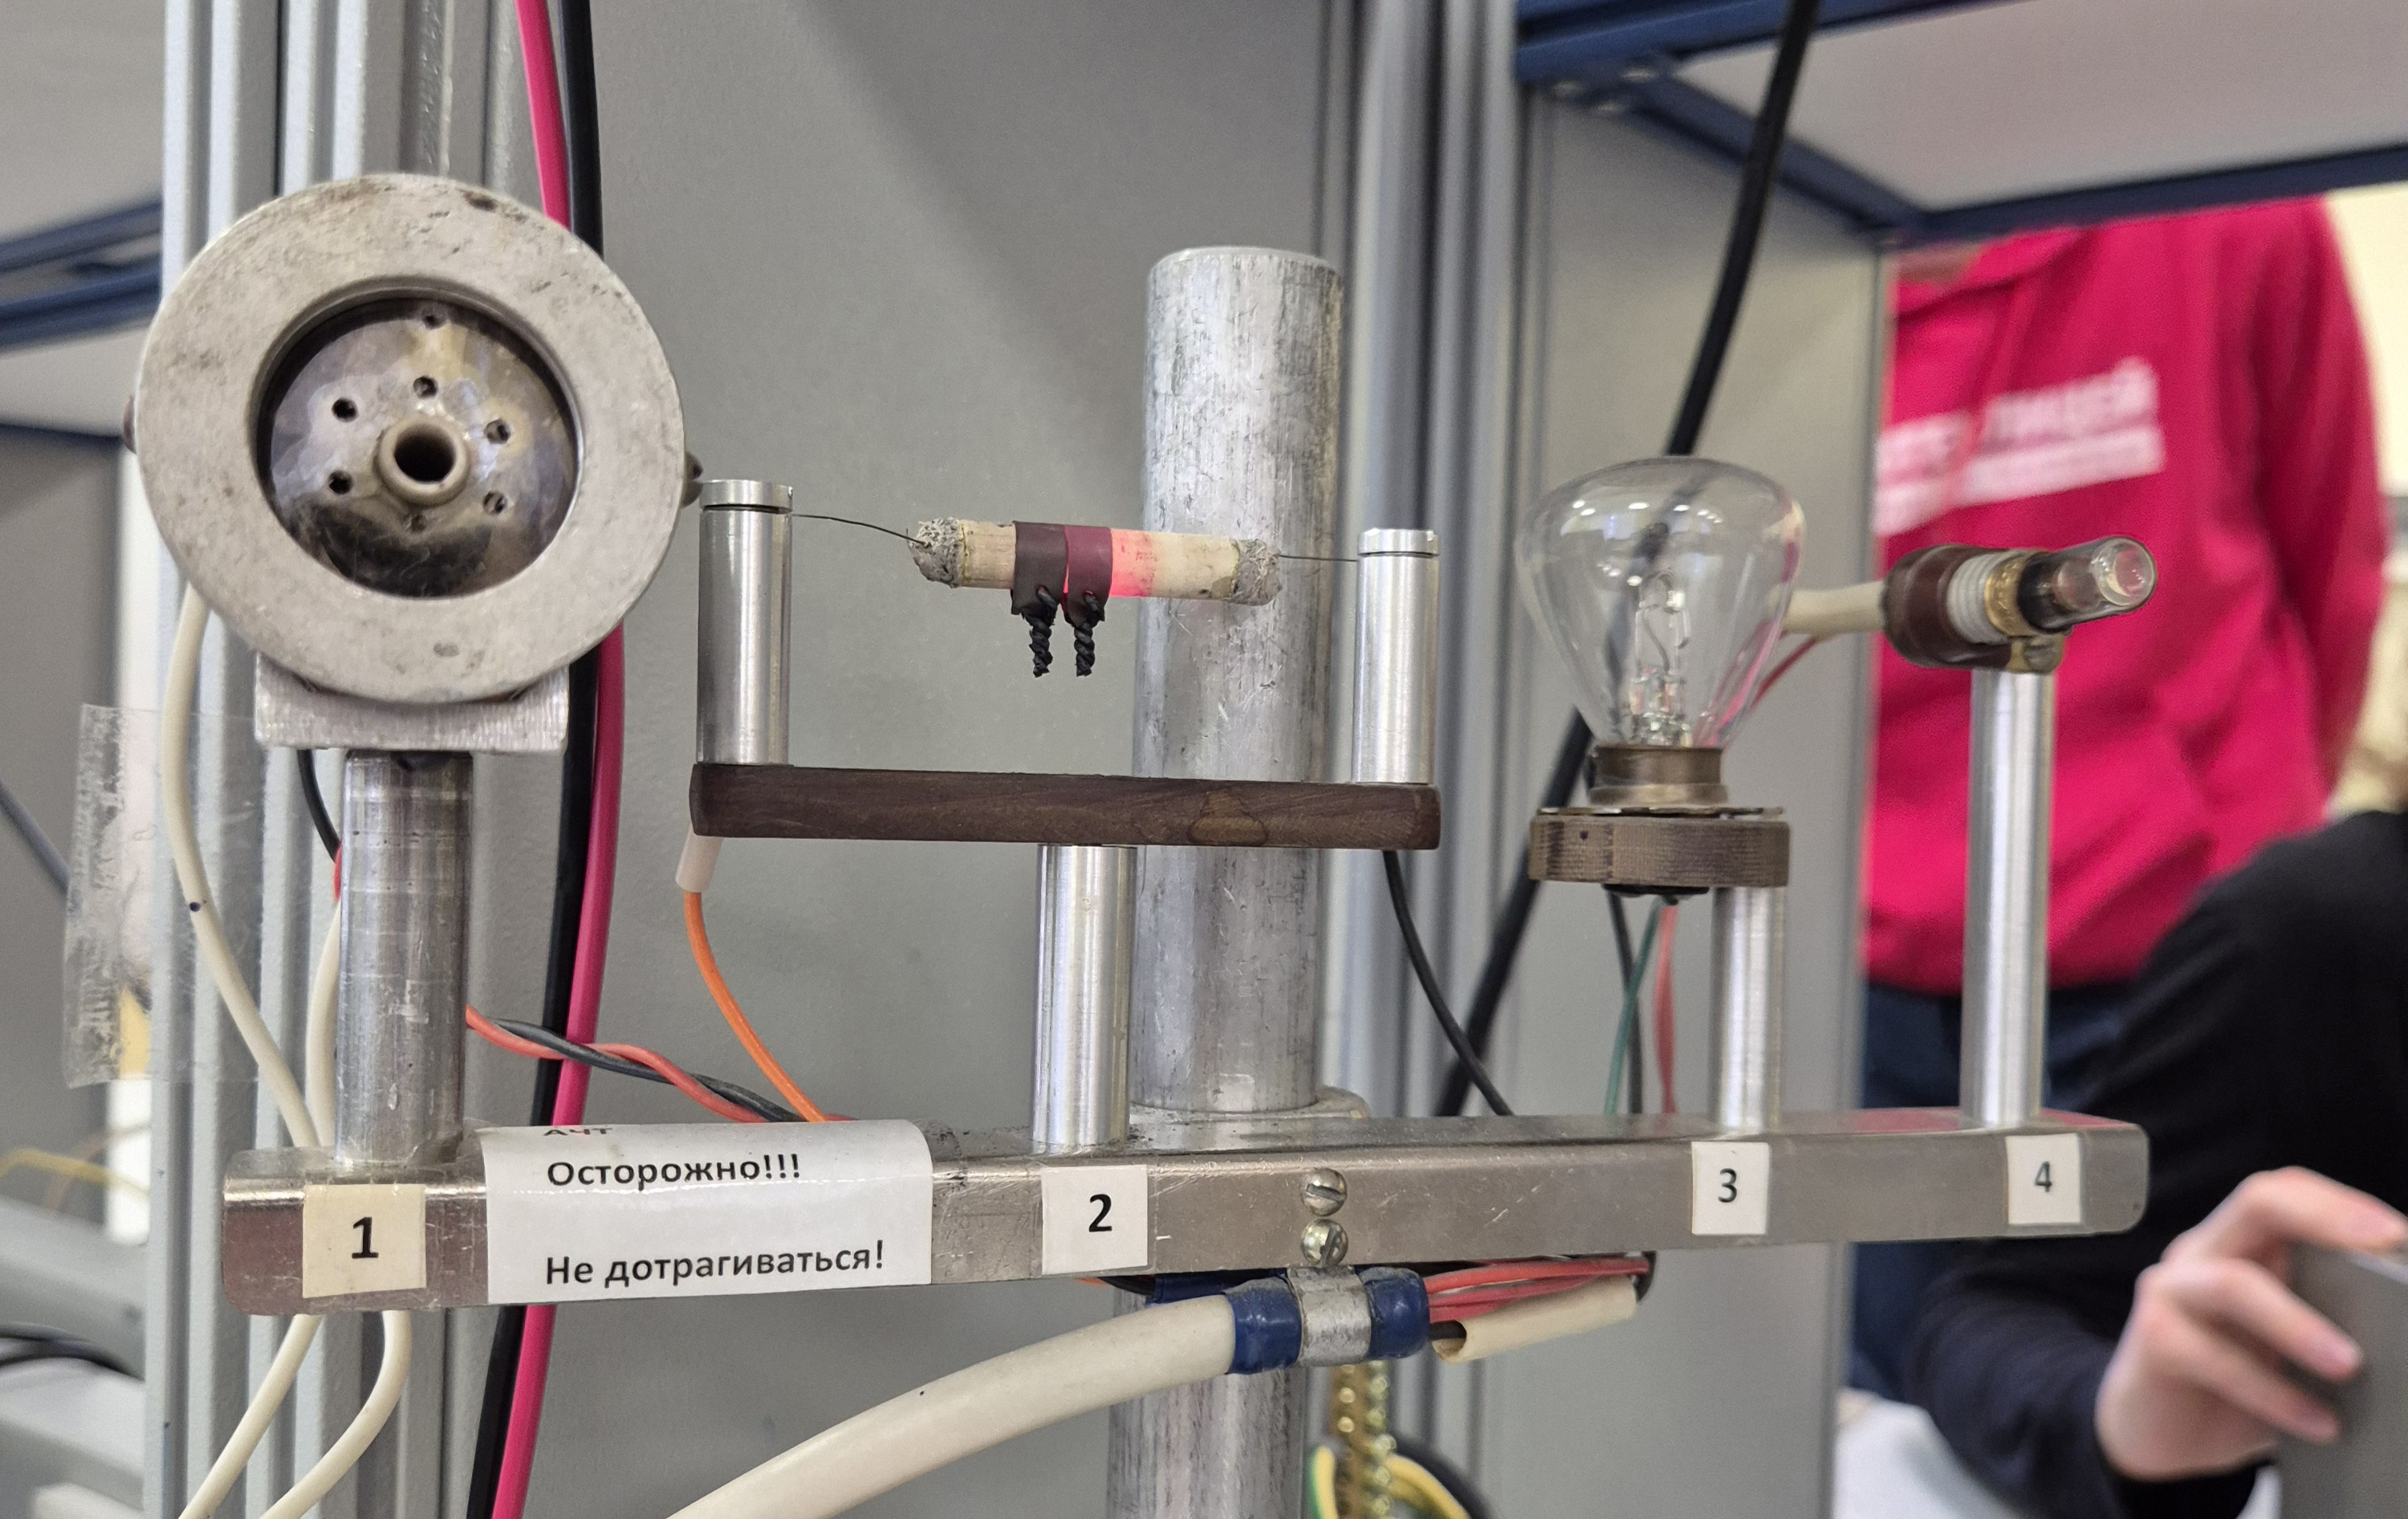
\includegraphics[width=.8\linewidth]{../images/581-4}
\caption{Общий вид исследуемых образцов}
\end{figure}


\section{Проведение эксперимента и обработка результатов}

\subsection{Опробование работы оптического пирометра}

Проведем измерения температуры АЧТ с помощью пирометра. Для этого нагреем модель АЧТ до красного каления. Перемещением объектива пирометра добъемся четкого изображения поверхности дна АЧТ. С помощью пирометра определим температуру АЧТ. Также запишем показания напряжения на термопаре, подключенной к АЧТ. По напряжению определим температуру АЧТ с помощью зависимости, представленной в описании к работе. Зависимость построена для комнатной температуры, равной $20\ ^\circ C$. Однако при выполнении температура в лаборатории была чуть выше -- $(23-24)\ ^\circ C$.

\begin{table}[H]
\centering
\begin{tabular}{|c|c|c|c|c|}
\hline
N & $T_1,\ ^\circ C$ & $U,\ мВ$  & $T_2,\ ^\circ C$ & $\Delta T/T_2,\ \%$\\ \hline
1 & 913  & 37.03 & 909  & 0.4 \\ \hline
2 & 913  & 36.92 & 906  & 0.8 \\ \hline
3 & 913  & 36.92 & 906  & 0.8 \\ \hline
4 & 907  & 36.72 & 901  & 0.7 \\ \hline
\end{tabular}
\end{table}

Как можно видеть по таблице, разница значений, полученных двумя различными методами, не превышает 1\%. Это говорит об исправной работе пирометра.
Также из проведенных изхмерений можно утверждать, что погрешность определения температуры с помощью пирометра приблизительно составляет $\sigma_T=5\ ^\circ C$. 

\subsection{Измерение яркостной температуры накаленных тел}

Направим пирометр на поверхность керамической трубки с кольцами из различных материалов. Нагреем трубку до темно-красного каления.
Измерим яркостную температуру трубки и каждого из колец.
\[T_{тр}=812\ ^\circ C,\quad T_{к1}=760\ ^\circ C,\quad T_{к2}<750\ ^\circ C\]
Различные яркостные температуры при одинаковой термодинамической объясняются отличием излучаемого телами спектра от планковского. То есть, исследуемые тела плохо соответствуют модели АЧТ.

\subsection{Проверка закона Стефана-Больцмана}

Направим пирометр на нить лампы накаливания. Постепенно увеличивая накал нити, будем фиксировать ее температуру с помощью пирометра. Так же запишем напряжение и величину тока на нити лампы при каждом измерении.

\begin{table}[H]
\centering
\begin{tabular}{|c|c|c|c|}
\hline
N & $T,\ ^\circ C$& $I,\ мА$ & $U,\ В$ \\ \hline
1 & 915 & 536.2 & 1.71 \\ \hline
2 & 1074 & 588.1 & 2.17 \\ \hline
3 & 1108 & 613.4 & 2.40 \\ \hline
4 & 1204 & 668.0 & 2.92 \\ \hline
5 & 1303 & 707.5 & 3.32 \\ \hline
6 & 1373 & 741.8 & 3.67 \\ \hline
7 & 1450 & 782.6 & 4.12 \\ \hline
8 & 1498 & 809.3 & 4.41 \\ \hline
9 & 1598 & 871.0 & 5.13 \\ \hline
10 & 1700 & 971.4 & 6.37 \\ \hline
11 & 1815 & 1066.4 & 7.66 \\ \hline
12 & 1899 & 1078.0 & 7.74 \\ \hline
\end{tabular}
\end{table}

Погрешности вольметра GDM-8135 определяются по формулам $\sigma_I=0.2\%+0.1\ мА$, $\sigma_I=0.1\%+0.01\ В$.

Для дальнейшей обработки так же понадобится зависимость коэффициента излучения $\varepsilon_{\lambda,\ T}$ от температуры. Она приведена в описании к работе в виде таблицы. Аппроксимируем ее линейной зависимостью для упрощения дальнейшей работы.

\begin{figure}[H]
\centering
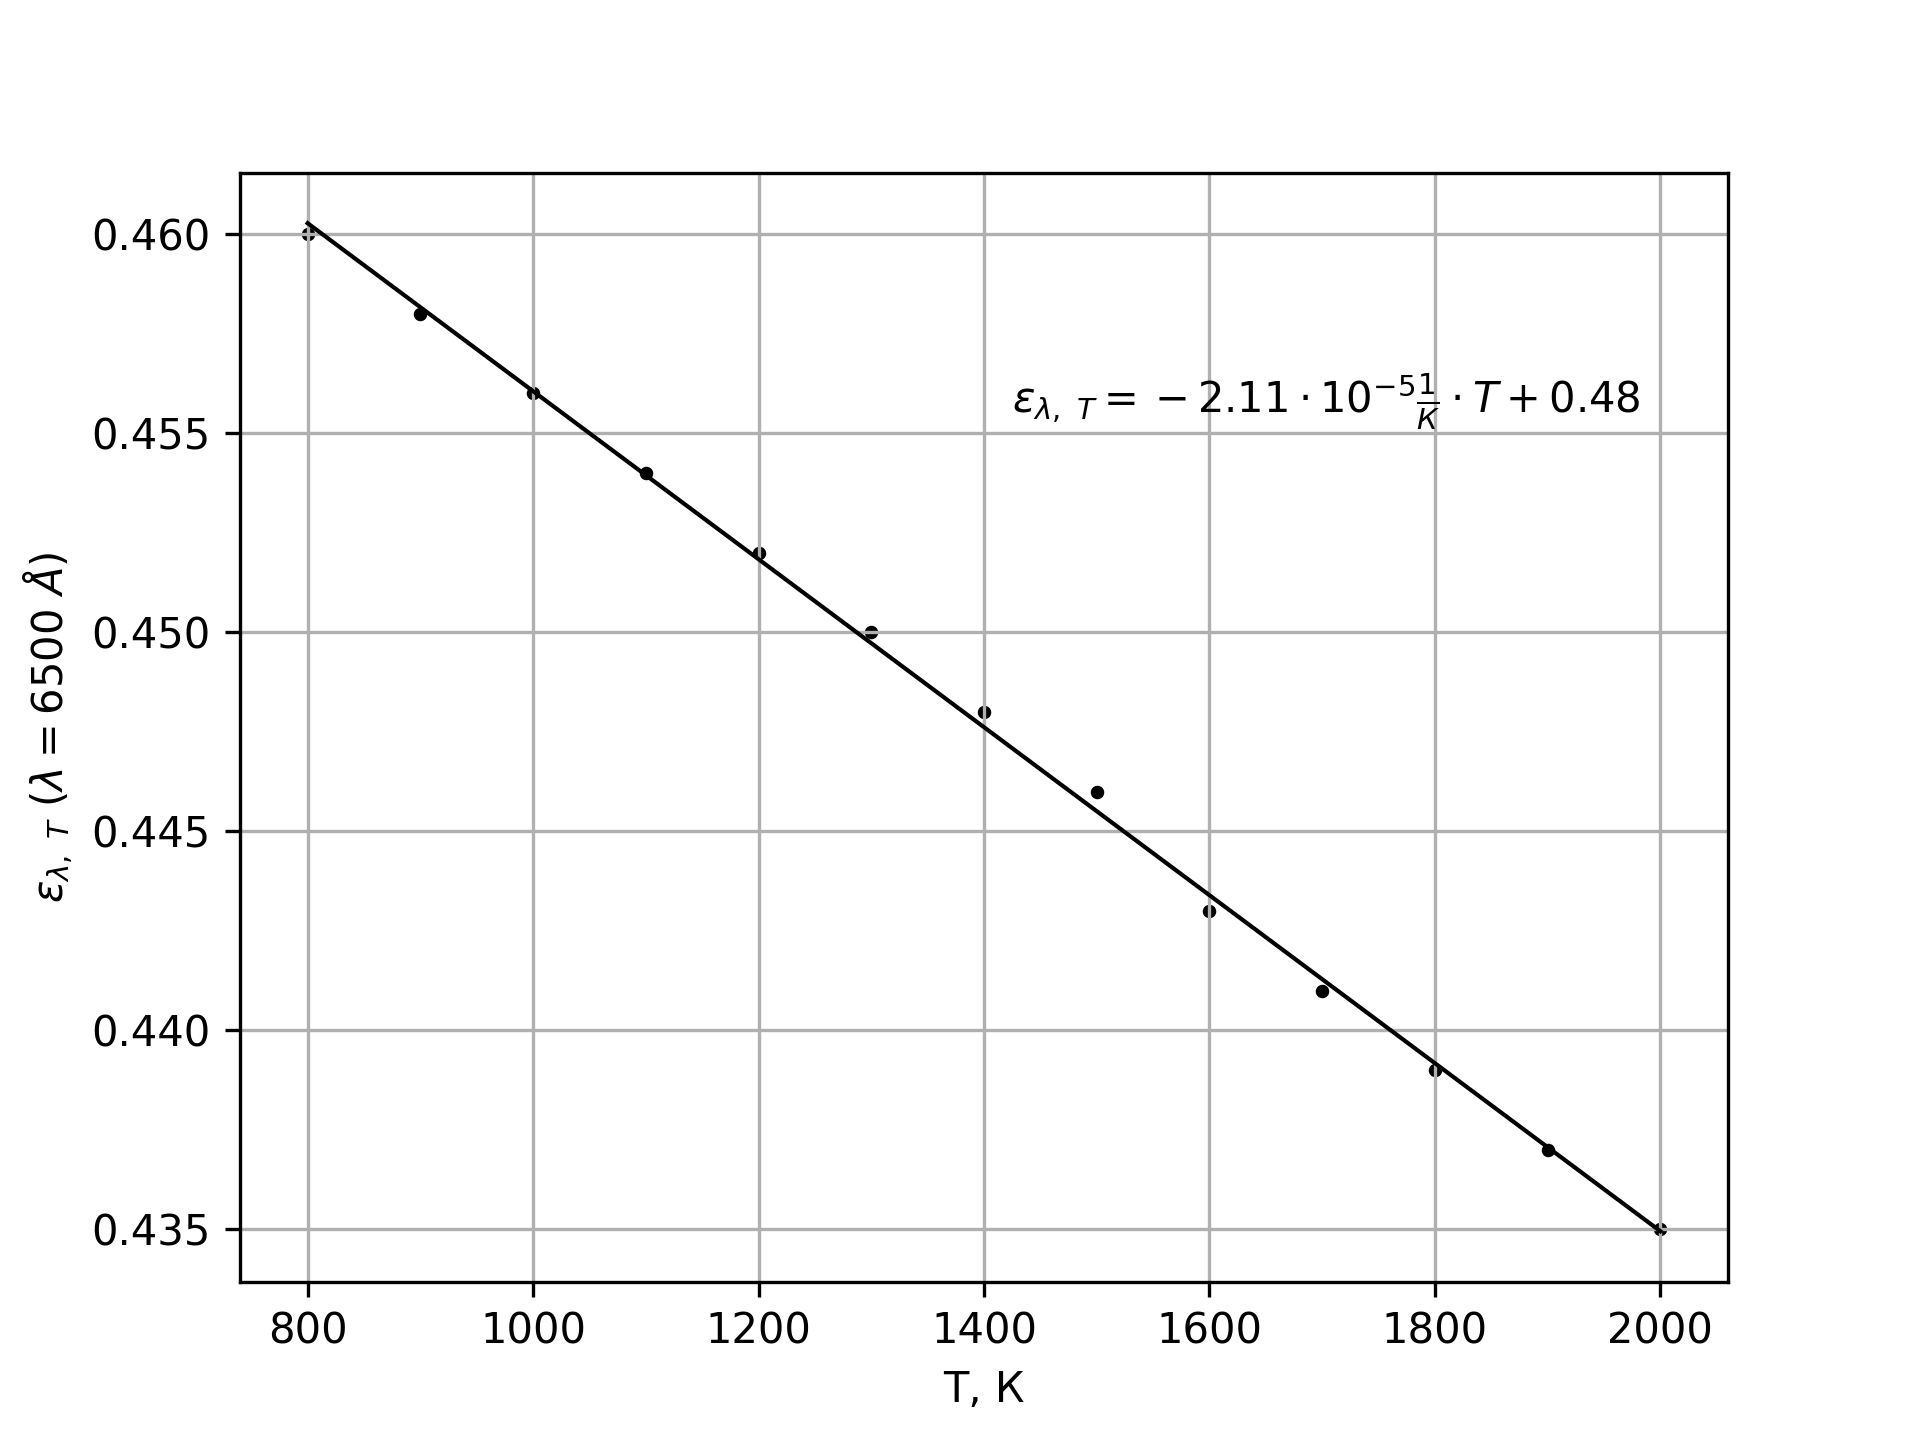
\includegraphics[width=.8\linewidth]{../images/581-1}
\caption{Зависимость коэффициента излучения от температуры}
\end{figure}

\newpage

Погрешность определения коэффициента из данной зависимости определяется с помощью матрицы ковариации.
\[\sigma_\varepsilon^2=|4.39\cdot10^{-14}\frac{1}{К^2}\cdot T^2-2\cdot 6.14\cdot10^{-11}\frac{1}{К}\cdot T+9.22\cdot10^{-8}|\]

Проверим выполнение закона Стефана-Больцмана.
\[W=UI=\varepsilon_{\lambda,\ T}S\sigma T^n\]
\[\ln{\frac{UI}{\varepsilon_{\lambda,\ T}}}=\ln{S\sigma}+n\ln{T}\]

\begin{figure}[H]
\centering
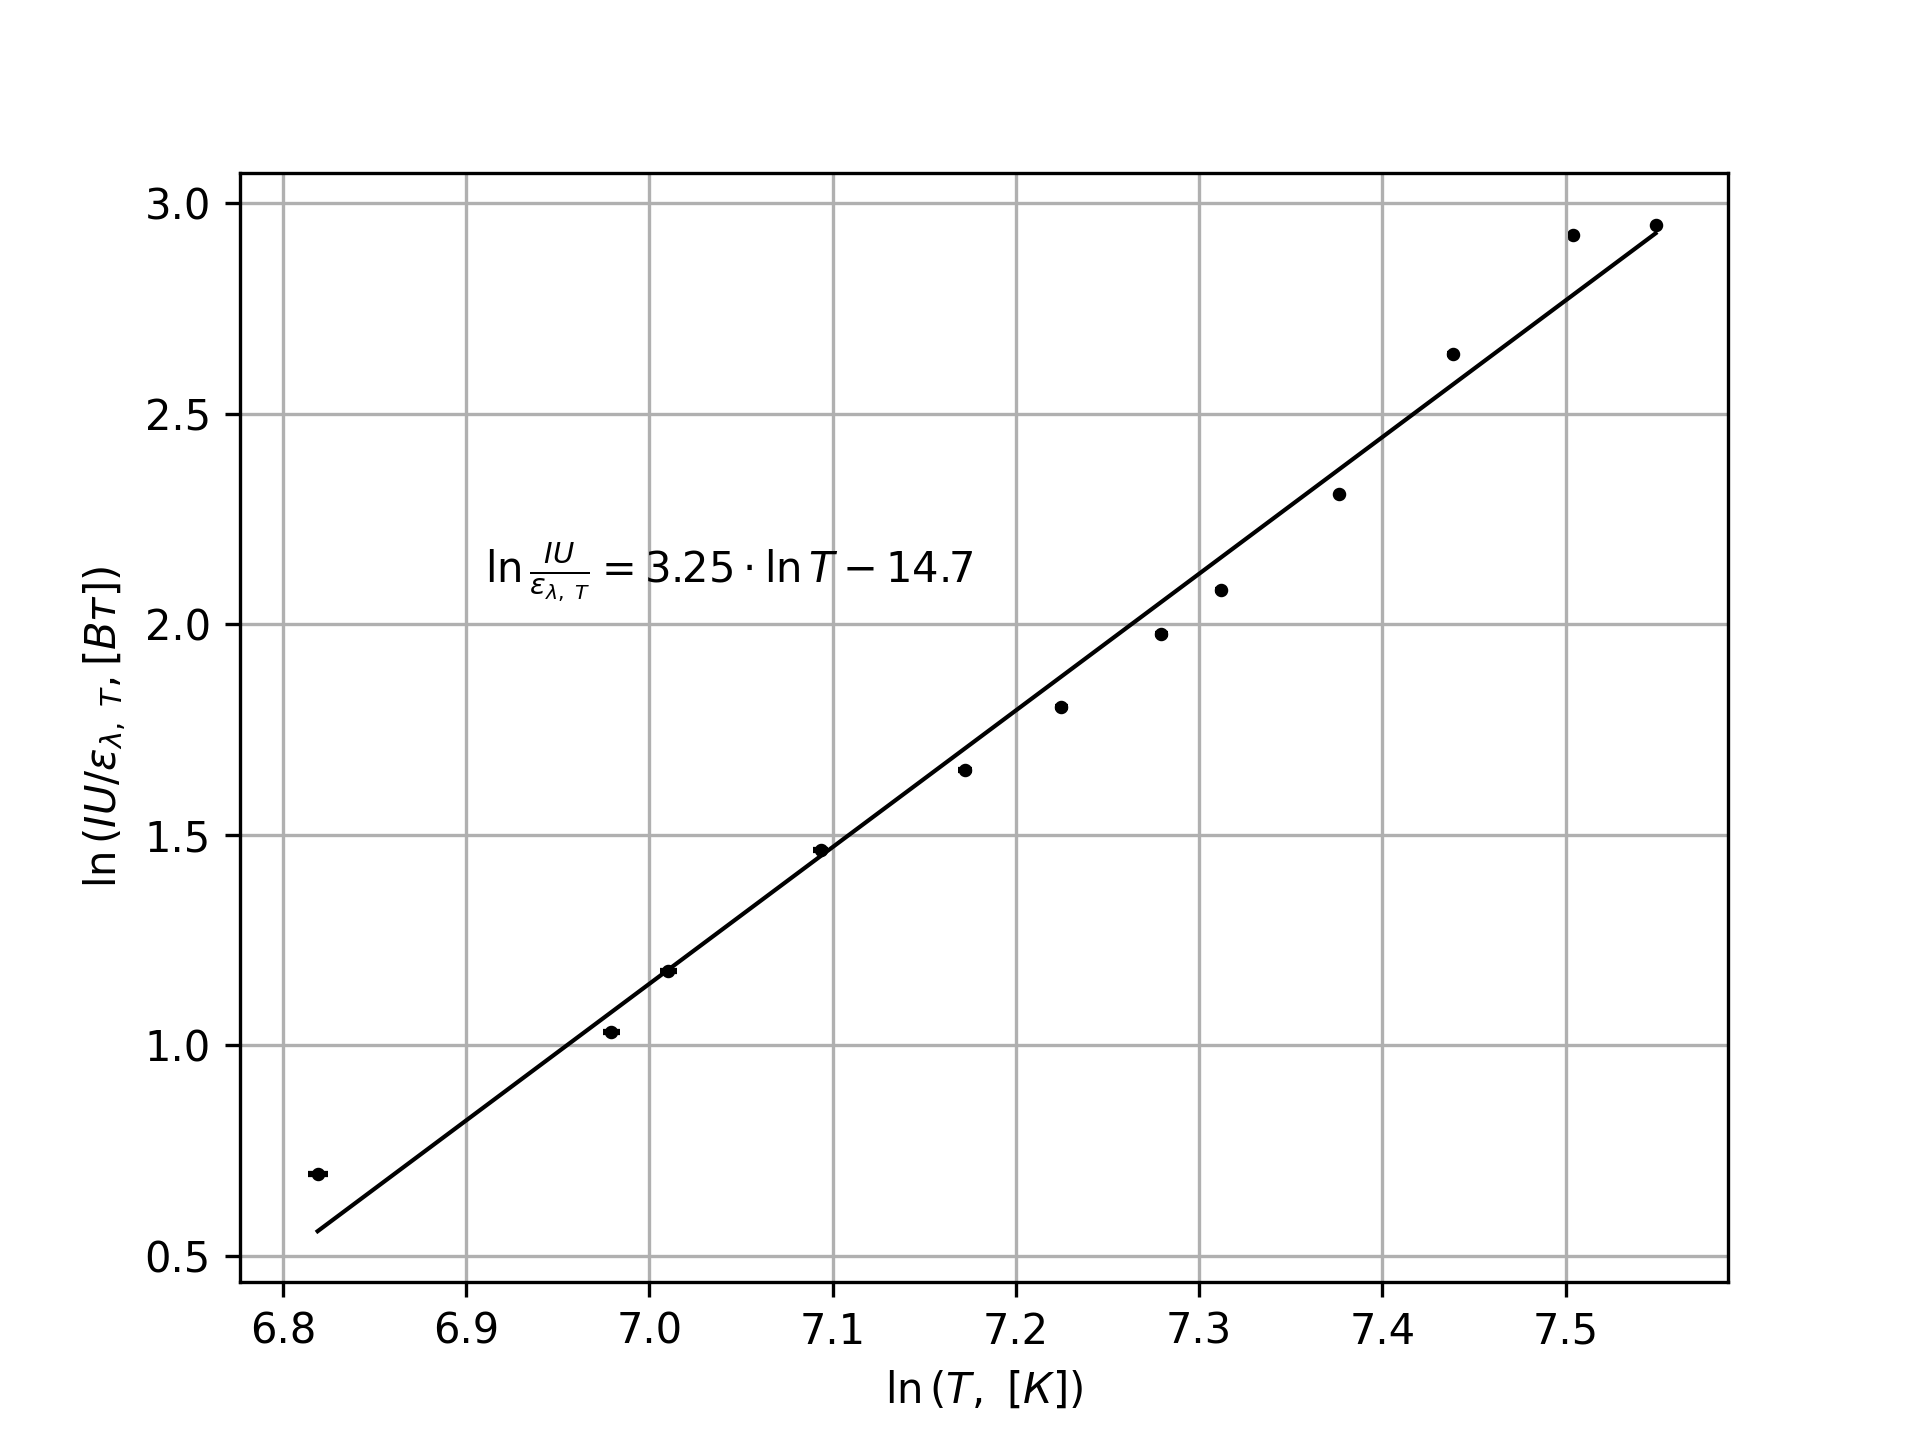
\includegraphics[width=.8\linewidth]{../images/581-2}
\caption{Зависимость мощности от температуры в логарифмическом масштабе}
\end{figure}

Построим последнюю зависимость. Получим, что $n=3.25\pm0.11$. Постоянную Стефана-Больцмана можно определить зная, что $S=0.36\ см^2$: $\sigma=(1.19\pm0.10)\cdot10^{-5}\ \frac{Вт}{м^2\cdot K^4}$.

\newpage

Также можно построить зависимость $W=UI$ от $\varepsilon_{\lambda,\ T}ST^4$.

\begin{figure}[H]
\centering
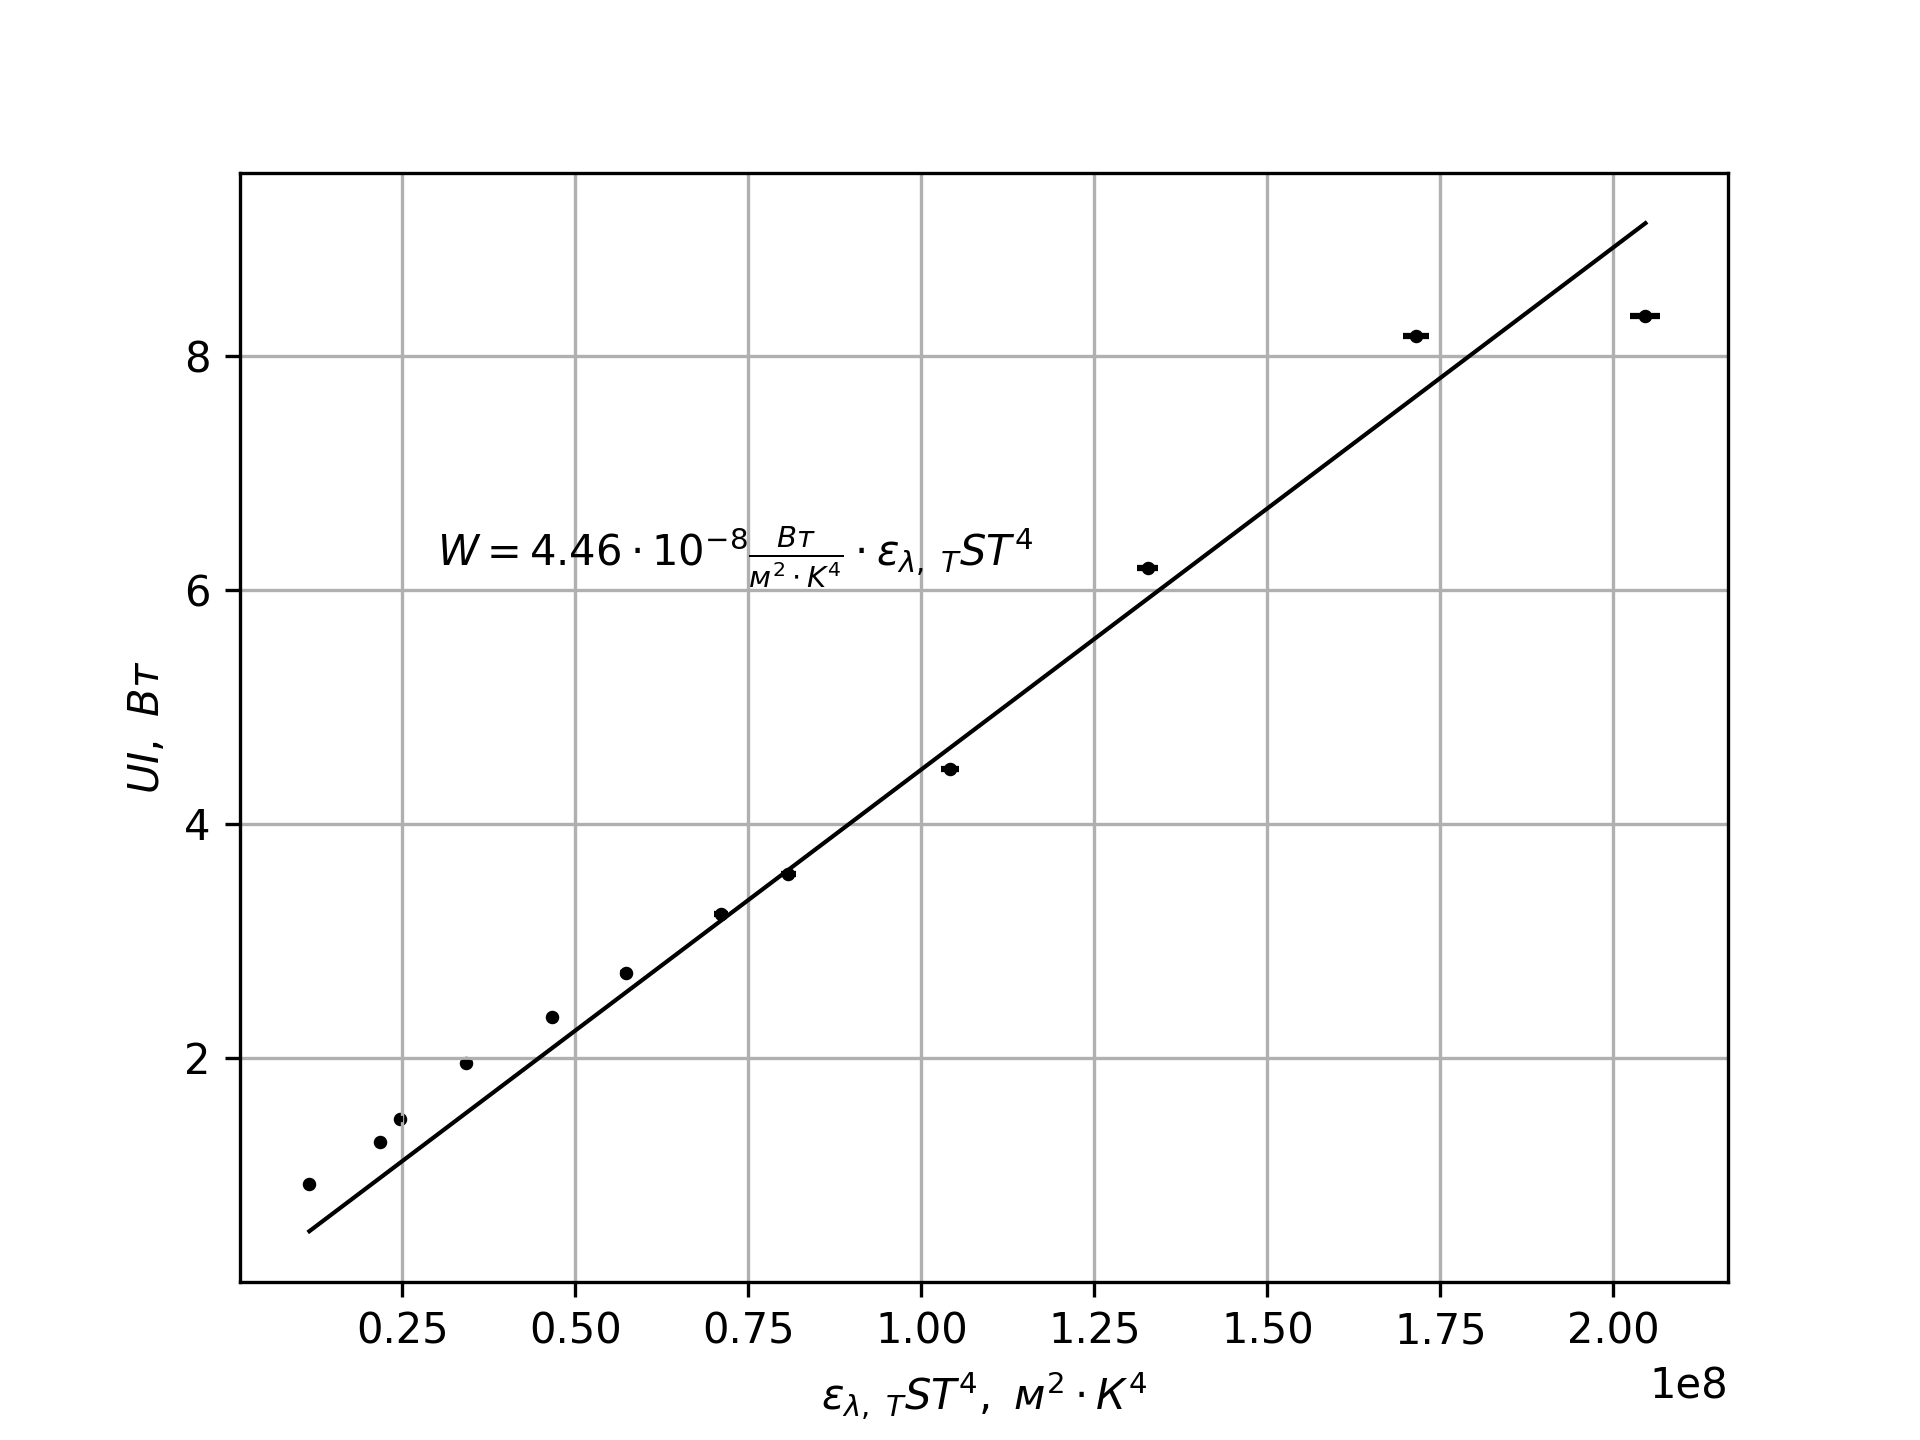
\includegraphics[width=.8\linewidth]{../images/581-3}
\caption{Зависимость $W(\varepsilon_{\lambda,\ T}ST^4)$}
\end{figure}

Угловой коэффициент проведенной прямой является постоянной Стефана-Больцмана.
\[\sigma=(4.46\pm0.11)\cdot10^{-8}\ \frac{Вт}{м^2\cdot K^4}\]

Можно отметить, что второй способ позволяет определить постоянную со значительно большей точностью.

По нему определим величину постоянной Планка по формуле:

\[h=\sqrt[3]{\frac{2\pi^5 k_Б^4}{15c^2\sigma}}=(7.17\pm0.06)\cdot10^{-34}\ Дж\cdot с\]

\subsection{Измерение «яркостной температуры» неоновой лампочки}

Направим пирометр на неоновую лампочку. «Яркостная температура» составляет $T_{ярк}=918\ ^\circ C$. Однако на ощупь температура лампочки является приблизительно комнатной. Столь завышенная яркостная температура объясняется присутствием интенсивных линий излучения неона в диапазоне спектра, используемого в работе.

\end{document}